\documentclass[]{article}
\usepackage{geometry}
 \geometry{
 a4paper,
 total={170mm,257mm},
 left=25mm,
 right= 35mm,
 top=25mm,
 bottom= 30mm
 }

\usepackage[T1]{fontenc}
\usepackage{lmodern}
\usepackage{amssymb,amsmath}
\usepackage{ifxetex,ifluatex}
\usepackage{fixltx2e} % provides \textsubscript
% use upquote if available, for straight quotes in verbatim environments
\IfFileExists{upquote.sty}{\usepackage{upquote}}{}
\ifnum 0\ifxetex 1\fi\ifluatex 1\fi=0 % if pdftex
  \usepackage[utf8]{inputenc}
\else % if luatex or xelatex
  \ifxetex
    \usepackage{mathspec}
    \usepackage{xltxtra,xunicode}
  \else
    \usepackage{fontspec}
  \fi
  \defaultfontfeatures{Mapping=tex-text,Scale=MatchLowercase}
  \newcommand{\euro}{€}
\fi

%%% Research Diary - Entry
%%% Template by Mikhail Klassen, April 2013
%%% 

% arara: pdflatex: { draft: true }
% arara: makeglossaries
% arara: pdflatex: { synctex: true }    
% arara: pdflatex: { synctex: true }  

% %titlesec subcaption subfigure
%\documentclass[11pt,letterpaper]{article}
\usepackage[spanish, english]{babel} % Manejo de idiomas
\usepackage{titlesec} % para anidar secciones
%\usepackage{subfiles}
%\usepackage[hidelinks,pagebackref,backref=page,linktocpage]{hyperref} % hide links 
%\usepackage[pagebackref, hypertexnames=false]{hyperref} % hide links 
%\hypersetup{linktocpage} % for links in toc. no es necesario,eliminaba otros enlaces
%\pdfstringdefDisableCommands
% \pdfstringdefDisableCommands to temporarily disable the command while the bookmark is written.
%http://www.dickimaw-books.com/cgi-bin/faq.cgi?action=view&categorylabel=glossaries
\usepackage{subcaption} % make subfigures
\usepackage{datetime}
\usepackage{cite}
%\usepackage{natbib}
\usepackage[utf8]{inputenc} %caracteres de la bibliografía
\newcommand{\mylib}{../library}
\usepackage{textcase} % Makelowercase...
\usepackage[toc,page]{appendix} % appendix and toc
\usepackage[acronym,toc,style=treenoname,order=word,subentrycounter]{glossaries}
%in subsection: acrfull instead of glsentryfull
%\renewcommand{\glscaption}{\robustify{\gls}}
%\robustify{\gls}% Make \gls not fragile
%\protect
\makeindex
\makeglossaries
%\makeglossaries main_page.tex
%\newcommand{\document}{\title}

\usepackage{comment}



\usepackage{mathrsfs,amsmath} 
\usepackage[makeroom]{cancel}
\usepackage{soul} % para que al subrayar no se salga de los márgenes
\usepackage{amsfonts} % for the \checkmark command 
% % % Cross mark
\usepackage{pifont}
\newcommand{\crossmark}{\hspace{1pt}\ding{55}}

\usepackage{enumitem} % personalized lists

%\usepackage{hyperref} % link to the page on the toc
\begin{comment}
\ersetup{
    colorlinks,
    citecolor=black,
    filecolor=black,
    linkcolor=black,
    urlcolor=black,
	linktocpage}
\end{comment}
\usepackage{graphicx} % includegraphics command is implemented here
\usepackage{csquotes} % in order to do citations  \blockcquote{bibid}{text}
\usepackage{amsmath}
\usepackage{mathtools}  % mathematical symbols. loads: \usepackage{amsmath}
\usepackage{amssymb}
\usepackage{tabularx} % multiple line equations (see SmithChart) http://tex.stackexchange.com/questions/33433/how-to-place-and-number-3-short-equations-in-one-line
\usepackage{steinmetz} % loads the phase function \phase
% % cleveref 
\usepackage[noabbrev]{cleveref} % noabbrev,capitalize,nameinlink
\crefformat{equation}{equation~#2#1#3}
\Crefformat{equation}{Equation~#2#1#3}
%newcommand{\workingDate}{\textsc{2013 $|$ January $|$ 01}}
%\usepackage{tabularx} % to adjust table widths
%Change pagewidth for tables
%\usepackage[showframe=true]{geometry}
%\usepackage[showframe=false]{geometry}
\usepackage{changepage}
%%\begin{adjustwidth}{-2cm}{} \end{adjustwidth}
% also
%\renewcommand{\tabcolsep}{4.6pt}
%\begin{tabular}{@{} *{21}{l} @{}} % use "@{}" suppresses whitespace at start and end of table
\newcommand{\userName}{Isabel María Villalba Jiménez}
\newcommand{\institution}{Universitat Politècnica de Catalunya}
% To add your univeristy logo to the upper right, simply
% upload a file named "logo.png" using the files menu above.

\usepackage[overload]{empheq}
\begin{comment}
		\begin{subequations}
		\begin{align}[left = \empheqlbrace\,]
		\begin{equation}
		\Delta \phi_1 \left(t\right)=\eta V_1 sin\left(\omega_m t\right)-\frac{\pi}{2}\\ 
		\end{equation}    
		\begin{equation}
		\Delta \phi_2 \left(t\right)=\eta V_2 sin\left(\omega_m t\right)\\
		\end{equation}			
		\end{align}
		\end{subequations}
\end{comment}

		
		
\sloppy % avoid exceeding right margin





		\begin{comment}
		% IMPORTANT
		\begin{align}
		E_{out}=&\left[------------\\
		&\left. --------------------\right.\\
		&\left. ------------------- \right] e^{j\omega_c t}		
		\label{eq:MZM_04}
		\end{align} 
		\end{comment}


\usepackage{url}
%\usepackage{underscore}
\usepackage[square, comma, numbers, sort]{natbib}
\bibliographystyle{unsrtnat}


% use microtype if available
\IfFileExists{microtype.sty}{\usepackage{microtype}}{}
\ifxetex
  \usepackage[setpagesize=false, % page size defined by xetex
              unicode=false, % unicode breaks when used with xetex
              xetex]{hyperref}
\else
  \usepackage[unicode=true]{hyperref}
  %\usepackage{hyperref}	
\fi
\hypersetup{breaklinks=true,
            bookmarks=true,
            pdfauthor={},
            pdftitle={},
            colorlinks=true,
            citecolor=blue,
            urlcolor=blue,
            linkcolor=magenta,
            pdfborder={0 0 0}}
\urlstyle{same}  % don't use monospace font for urls
\setlength{\parindent}{0pt}
\setlength{\parskip}{6pt plus 2pt minus 1pt}
\setlength{\emergencystretch}{3em}  % prevent overfull lines
\setcounter{secnumdepth}{2}


\author{}
\date{}

% Set roman section numbering
\renewcommand{\thesection}{\Roman{section}.} 
\renewcommand{\thesubsection}{\thesection \Roman{subsection}}


\newcommand{\competition}{The Marinexplore and Cornell University Whale Detection Challenge}
\newcommand{\imagenet}{ImageNet Large Scale Visual Recognition Competition (ILSVRC)}
\newcommand{\copyrighting}{“Copyright © 2011 by Cornell University and the Cornell Research Foundation, Inc. All Rights Reserved”}
\title{Capstone Project: \\ Right Whale call recognition using \\ Convolutional Neural Networks}\label{capstone-project}



\begin{document}
\maketitle

\section*{Machine Learning Engineer Nanodegree}\label{machine-learning-engineer-nanodegree}

Isabel María Villalba Jiménez \\ \today

\section{Definition}\label{i.-definition}

\emph{(approx. 1-2 pages)}

\subsection{Project Overview}\label{project-overview}

%In this section, look to provide a high-level overview of the project in layman's terms. Questions to ask yourself when writing this section: - \emph{Has an overview of the project been provided, such as the problem domain, project origin, and related datasets or input data?} - \emph{Has enough background information been given so that an uninformed reader would understand the problem domain and following problem statement?}

Right whales are one of the most endangered species around the world, with only a few 400 remaining. Many of casualties among them are caused by crashing into boats. One way of avoiding these collisions is to alert ships when whales are detected in the proximity.

In order to do so, Cornell University's Bioacoustic Research Program, which has extensive experience in identifying endangered whale species, has deployed a 24/7 buoy network to guide ships from colliding with the world's last 400 North Atlantic right whales.

This work comes from a proposal of the Cornell University's Bioacoustic Research Program of finding new ways of improving the detection of these mammals through the audio signal of the buoys network.  Cornell University provides for the competition a dataset with recordigs made by the buoys. The proposal was made through a Kaggle competition named \href{https://www.kaggle.com/c/whale-detection-challenge}{\competition} \cite{kagglewhale} \copyrighting.

\subsection{Problem Statement}\label{problem-statement}

\begin{comment} 
In this section, you will want to clearly define the problem that you are trying to solve, including the strategy (outline of tasks) you will use to achieve the desired solution. You should also thoroughly discuss what the intended solution will be for this problem. Questions to ask yourself when writing this section: - \emph{Is the problem statement clearly defined? Will the reader understand what you are expecting to solve?} - \emph{Have you thoroughly discussed how you will attempt to solve the problem?} - \emph{Is an anticipated solution clearly defined?  Will the reader understand what results you are looking for?}
\end{comment}
Right whales make a half-dozen types of sounds, but the most characteristic one is the up-call. This type of "contact call",  is a little like small talk-- the sound of a right whale going about its day and letting others know it is nearby. In figure \ref{img:upcall} it is represented the spectrogram of an up-call which sounds like a deep, rising “whoop” that lasts about a second (sound in \cite{CornellWeb}, other calls in \cite{CornellWeb2}).

\begin{figure}[htpb!]
\centering
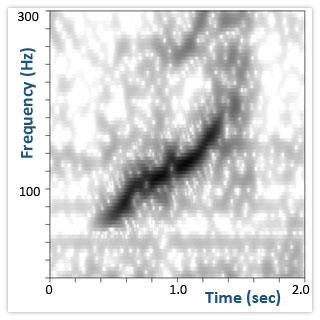
\includegraphics[width= 0.3\textwidth]{images/sound_upcall_quiet.jpg}
\caption{Spectrogram of a rigth whale up-call \cite{CornellWeb} \label{img:upcall}}
\end{figure}
The goal of this work is to present a model capable of detecting the right whale's up-call, which is the most characteristic call of this specie, from the audio detected by the buoys deployed in the sea.

Impressed by the working principle of Convolutional Neural Networks, I decided looking for uses beyond pure image classification. I also had been wondering if anything related to animals and whales could be done. I started looking in the internet and found several Kaggle competitions: one on whale detection through images (\href{https://www.kaggle.com/c/noaa-right-whale-recognition}{Right Whale Recognition}), and other on recognizing the North Atlantic Right Whale call (\href{https://www.kaggle.com/c/whale-detection-challenge}{\competition}). Searching for applications of Convolutional Neural Networks in sound recognition, I found an entry related to the \competition. In \cite{Nouriblog} Daniel Nouri proposed to use ConvNets not just to go across the spectrogram of the whale calls, but try to recognize a pattern by simply looking at its image, like a human could. With this proposal he got pretty good results with a very straight forward approach. I decided to give it a try and look for most used ConvNets schemes and see their performance in this competition.

The \textbf{workflow} can be organized as follows:
\begin{enumerate}
	\item sound samples exploration
	\item spectrogram generation and image processing (contrast, appropriate dimensions...)
	\item separation of dataset into training, cross-validation and test dataset and save into pickle 
	\item select ConvNets model and adjust parameters
	\begin{itemize}
		\item define structure of the ConvNet adequate for the images: depth of layers, and stride and patch size of filters and pooling layers
		\item AUC vs epochs (or training iterations), Error vs epochs, for different batch sizes
		\item tune the model using regularization and decaying learning rate		
	\end{itemize}
	\item compare the performance of winning model using the reduced version train and test dataset extracted form the train dataset
\end{enumerate}

\subsection{Metrics}\label{metrics}
\begin{comment} 
In this section, you will need to clearly define the metrics or
calculations you will use to measure performance of a model or result in your project. These calculations and metrics should be justified based on the characteristics of the problem and problem domain. Questions to ask yourself when writing this section: - \emph{Are the metrics you've chosen to measure the performance of your models clearly discussed and defined?} - \emph{Have you provided reasonable justification for the metrics chosen based on the problem and solution?}
\end{comment}

The main evaluation metric for this project will be that used in the Kaggle competition, this is the \textbf{Area Under the Curve (AUC)}, where the Curve is the ROC curve.

The \textbf{receiver operating characteristic (ROC)} curve is a graphical plot that illustrates the performance of a binary classifier system as its discrimination threshold is varied. The curve is created by plotting the true positive rate (TPR) against the false positive rate (FPR) at various threshold settings.

The true-positive rate is also known as sensitivity, recall or probability of detection. The false-positive rate is also known as the fall-out or probability of false alarm. 

The ROC curve is thus, the sensitivity as a function of fall-out. In general, if the probability distributions for both detection and false alarm are known, the ROC curve can be generated by plotting the cumulative distribution function (area under the probability distribution from $-\infty$  to the discrimination threshold) of the detection probability in the y-axis versus the cumulative distribution function of the false-alarm probability in x-axis (see figure \ref{img:ROC})\cite{wikiROC}

\begin{figure}[htpb!]
\centering
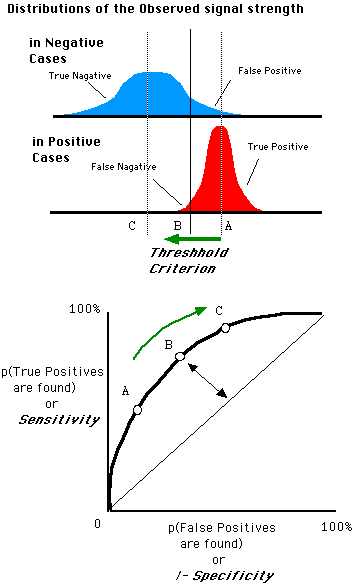
\includegraphics[width= 0.4\textwidth]{images/ROCfig}
\caption{ROC curve graphic explanation \cite{wikiwand} \label{img:ROC}}
\end{figure}

Another important measure can be the \textbf{error rate} vs iterations for a different batch sizes. The error rate used can be the percentage of wrong classified samples.

It can be also interesting to use the \textbf{confusion matrix}, which is a more detailed version of the ROC curve. The confusion matrix is a table that shows the predicted labels for each of the true input labels.

\section{Analysis}\label{ii.-analysis}

\emph{(approx. 2-4 pages)}
\subsection{Data Exploration}\label{data-exploration}
\begin{comment}
In this section, you will be expected to analyze the data you are using for the problem. This data can either be in the form of a dataset (or datasets), input data (or input files), or even an environment. The type of data should be thoroughly described and, if possible, have basic statistics and information presented (such as discussion of input features or defining characteristics about the input or environment).
Any abnormalities or interesting qualities about the data that may need to be addressed have been identified (such as features that need to be transformed or the possibility of outliers). Questions to ask yourself when writing this section: - \emph{If a dataset is present for this problem, have you thoroughly discussed certain features about the dataset? Has a data sample been provided to the reader?} - \emph{If a dataset is present for this problem, are statistics about the dataset calculated and reported? Have any relevant results from this calculation been discussed?} - \emph{If a dataset is \textbf{not} present for this problem, has discussion been made about the input space or input data for your problem?} - \emph{Are there any abnormalities or characteristics about the input space or dataset that need to be addressed? (categorical variables, missing values, outliers, etc.)}
\end{comment}

The dataset used comes from the competition and consists of 30,000 training samples and 54,503 testing samples. Each candidate is a 2-second .aiff sound clip with a sample rate of 2 kHz. The file "train.csv" gives the labels for the train set. Candidates that contain a right whale call have label=1, otherwise label=0. These clips contain any mixture of right whale calls, non-biological noise, or other whale calls \cite{CornellWeb, CornellWeb2}. 

The training dataset is imbalanced, consisting of approximately 7000 Right Whales samples and 23000 non right whales samples (figure \ref{img:train_dataset}). In order to deal with this problem, I could just balance the samples used (get the same amount of labels from each type) or try to use an algorithm that penalizes this imbalance.

\begin{figure}[htpb!]
\centering
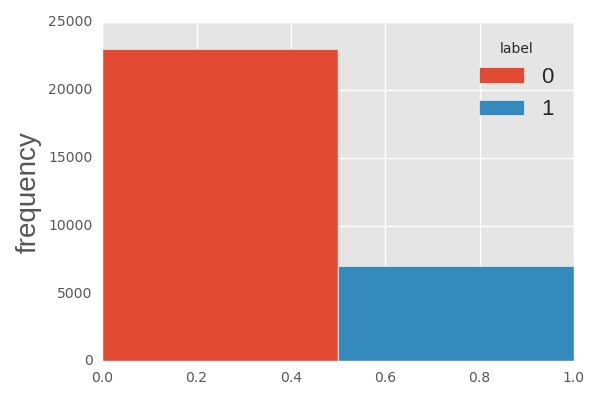
\includegraphics[width= 0.65\textwidth]{./images/2_dataset}
\caption{Dataset distribution \label{img:train_dataset}}
\end{figure}


\subsubsection{Exploratory Visualization}\label{exploratory-visualization}
\begin{comment}
In this section, you will need to provide some form of visualization
that summarizes or extracts a relevant characteristic or feature about the data. The visualization should adequately support the data being used. Discuss why this visualization was chosen and how it is relevant.
Questions to ask yourself when writing this section: - \emph{Have you visualized a relevant characteristic or feature about the dataset or input data?} - \emph{Is the visualization thoroughly analyzed and discussed?} - \emph{If a plot is provided, are the axes, title, and datum clearly defined?}

- Compare spectrogram of some non whale to some whales and then explain why I trimmed it
\end{comment}
The audio is recorded after the buoys auto-detect the characteristic up-call, what biases the dataset to that kind of calls. Thus, it makes sense to detect only the up-call, which is the most characteristic and most frequently emitted call (details on the deployment of the buoys and how the recordings are made in \cite{McDonald2002}). 

In figure \ref{img:samples}, samples corresponding to right-whale up-call (label = 1) show the that the energy of the signal is below 250Hz (see figure \ref{img:upcall}) and they exhibit a clear pattern. This fact will help to reduce information processed to that range of frequencies. 
In the second row, corresponding to negative identifications (label = 0) this pattern is not present. However, some samples from from other whale species or corresponding to right-whale making other calls are included in the label 0. This could be the case of sample train6776 in figure \ref{img:samples}.

Recordings have a duration of 1.8 seconds and a sampling rate of 2000 Hz. The raw spectrogram of the recordings result in images of 129x23 pixels.

\begin{figure}[htpb!]
\centering
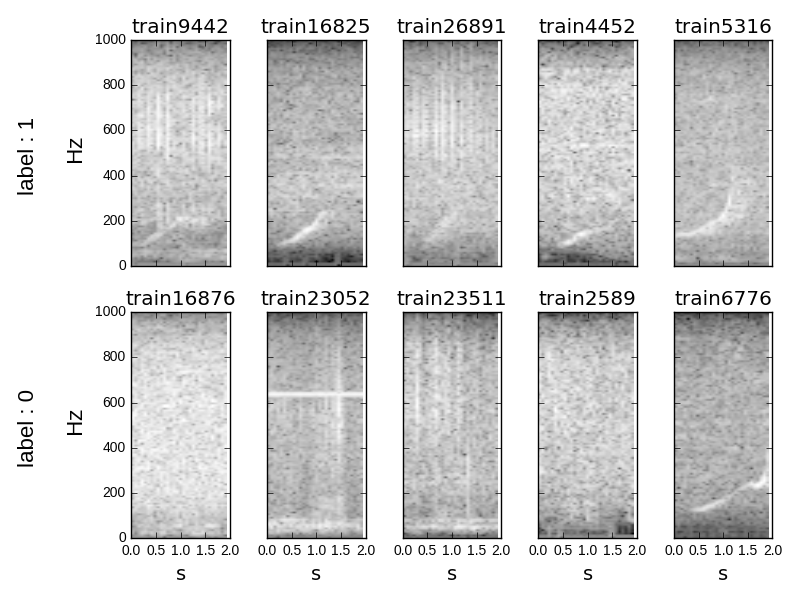
\includegraphics[width= \textwidth]{./images/2_samples}
\caption{Samples for right whale up-call (label 1) and no-right-whale up-call (label 0).  \label{img:samples}}
\end{figure} 


\subsubsection{Algorithms and
Techniques}\label{algorithms-and-techniques}
\begin{comment}
In this section, you will need to discuss the algorithms and techniques you intend to use for solving the problem. You should justify the use of each one based on the characteristics of the problem and the problem domain. Questions to ask yourself when writing this section: - \emph{Are the algorithms you will use, including any default variables/parameters in the project clearly defined?} - \emph{Are the techniques to be used thoroughly discussed and justified?} - \emph{Is it made clear how the input data or datasets will be handled by the algorithms and techniques
chosen?}
-- Maybe : logistic and SVM?
\end{comment}
In order to perform the prediction I will try to implement well-known and widely-implemented models of ConvNets.

Convolutional Neural Networks (ConvNets) are a type of Neural Networks (NNs) that make the assumption that inputs are images. This allows to encode certain properties into the architecture that make the forward function more efficient to implement and vastly reduce the amount of parameters in the network \cite{cs231convnets}.
ConvNets, like other NNs, are made up of layers. These layers (called hidden layers) transform input 3D volumes to output 3D volumes with some differentiable function that may or may not have parameters \cite{cs231convnets}. This is an interesting property of ConvNets: layers have neurons arranged in 3 dimensions (width, height and depth) (see figure \ref{img:cnn}). %Each hidden layer is made up of neurons, where each neuron is fully connected to all neurons in the previous layer, and where neurons in a single layer function completely independently and do not share any connections. The last fully-connected layer is called the “output layer” and in classification settings it represents the class scores. 

There are three main types of layers that are used to build ConvNets \cite{cs231convnets}: % Convolutional Layer, Pooling Layer, and Fully-Connected Layer .
\begin{itemize}
	\item Convolutional Layer (CONV): computes the output of neurons connected to local regions of the input, performing the dot product between their weight and a small region that are connected to. If the input is 3D (i.e. an image with RGB colors) this layer will also be 3-dimensional. Four hyperparameters control the size of the output volume: the depth, filter size, stride and zero-padding. Depth (D) is related to the number of filters used in the layer, the filter or patch have dimensions (F) (i.e. 2x2) and stride (S) is referred to the displacement of the filter. The amount Zero-padding (P), which allows to control the spatial size of outputs.
	\item Pooling Layer (POOL) (or Subsampling Layer): performs downsampling operation along spatial dimensions. Can be max-pooling (taking the maximum of a region), average-pooling (taking the average of a region) or other types of results from applying a function to a region of the image. It has two main hyperparameters: the spatial extent of the filter or patch where pooling is applied (F) and the stride (S) of this filter.
	\item Fully-Connected Layer (FC): is the same type of layer as in NNs.
\end{itemize}

Usually a CONV layer is followed by a RELU layer, which perform an elmentwise activation function (i.e. max(0,x),logistic function, tanh).

\begin{figure}[htpb!]
\centering
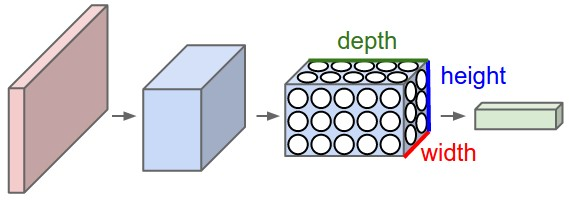
\includegraphics[width= 0.5\textwidth]{images/cnn}
\caption{ConvNet structure \cite{cs231convnets}\label{img:cnn}}
\end{figure}


LeNet is one of the first successful applications of Convolutional Networks were developed by Yann LeCun in 1990’s. One of the versions of LeNet is LeNet-5, used for handwritten and machine-printed character recognition. Figure \ref{img:lenet5} shows the structure of the network, composed of 2 convolutional layers, 2 fully connected layers and 2 subsampling or pooling layers. The layers follow the sequence: INPUT -> CONV -> RELU -> SUBS (POOL) -> CONV -> RELU -> SUBS (POOL) -> FC -> RELU -> FC, for INPUT, CONV, RELU, SUBS, FC. % meaning respectively the Input, Convolutional, RELU, Subsampling (or max pooling) and Fully Connected layer.
%\pagebreak
\begin{figure}[htpb!]
\centering
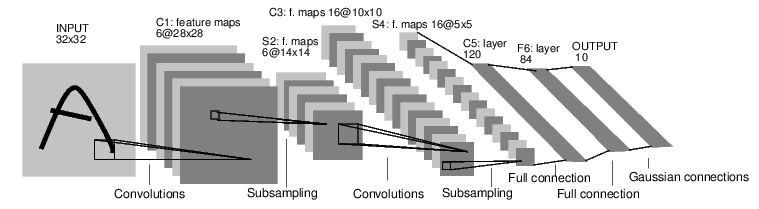
\includegraphics[width= 0.99\textwidth]{images/lenet5}
\caption{LeNet-5 structure \cite{Lecun98} \label{img:lenet5}}
\end{figure}

Other more complex ConvNet is AlexNet, developed by Alex Krizhevsky et al. \cite{Krizhevsky12}. The AlexNet was submitted to the ImageNet ILSVRC challenge in 2012 and significantly outperformed the second runner-up (top 5 error of 16\% compared to runner-up with 26\% error). It has a very similar architecture to LeNet, but it is  deeper, bigger, and features Convolutional Layers stacked on top of each other (previously it was common to only have a single CONV layer always immediately followed by a POOL layer)\cite{cs231convnets}. Figure \ref{img:imagenet12} shows the structure of the network, composed of 5 convolutional layers, 3 fully connected layers and 3 subsampling or pooling layers. The layers follow the sequence: INPUT -> CONV -> RELU -> SUBS -> CONV -> RELU -> SUBS -> CONV -> RELU -> CONV -> RELU -> SUBS -> FC -> RELU -> FC. %, for INPUT, CONV, RELU, SUBS, FC meaning respectively the Input, Convolutional, RELU, Subsampling (or max pooling) and Fully Connected layer .% Cambiar, LITERAL!


\begin{figure}[htpb!]
\centering
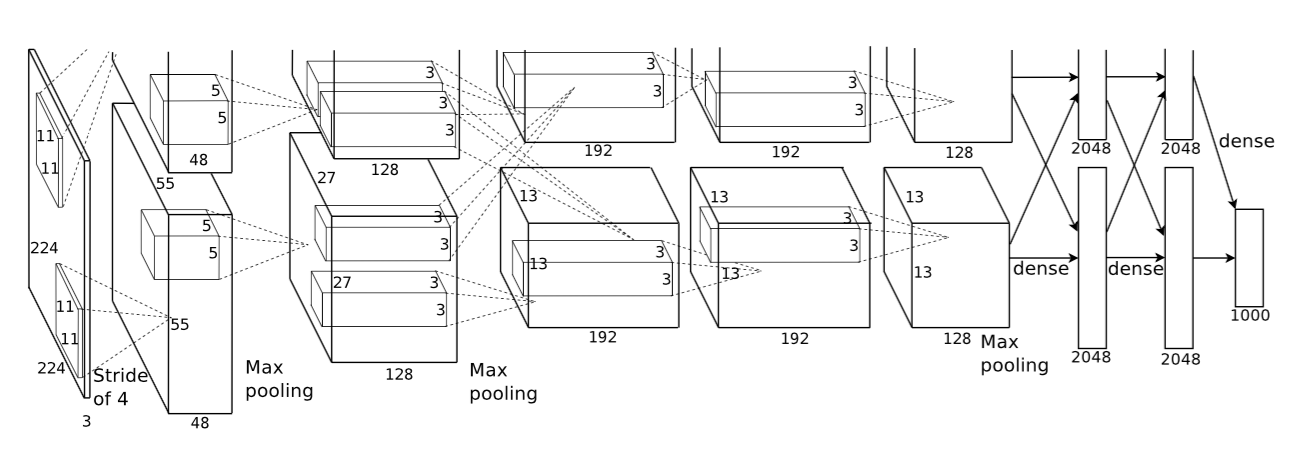
\includegraphics[width= 0.99\textwidth]{images/imagenet12}
\caption{Network structure by Krizhevsky \cite{Krizhevsky12} \label{img:imagenet12}}
\end{figure}

Some parameters need adjustment to adequate the network to this work, like the size of the patch (F) and stride (S) of the convolutional and pooling layers, and also the depth (D) of each convolutional layer. %This issue will be discussed in later sections.

\subsubsection{Benchmark}\label{benchmark}
\begin{comment}
In this section, you will need to provide a clearly defined benchmark result or threshold for comparing across performances obtained by your solution. The reasoning behind the benchmark (in the case where it is not an established result) should be discussed. Questions to ask yourself when writing this section: - \emph{Has some result or value been provided that acts as a benchmark for measuring performance?} - \emph{Is it clear how this result or value was obtained (whether by data or by hypothesis)?}
\end{comment}

I will try to compare the performance of popular ConvNets (i.e. LeNet-5 proposed by Lecun \cite{Lecun98} or AlexNet, the winner of the 2010 and 2012 \imagenet \, proposed by Krizhevsky \cite{Krizhevsky12}) with the performance of the winning model of the competition which is based on Gradient Boosting (SluiceBox: \href{https://github.com/nmkridler/moby}{Github}) and the Daniel Nouri's model based on Krizhevsky's 2012 ILSVRC ConvNet model \cite{Krizhevsky12} (\href{https://speakerdeck.com/dnouri/practical-deep-neural-nets-for-detecting-marine-mammals/}{source}), which first inspired this work.

The Area Under the Curve (AUC) (see the Evaluation metrics section \ref{evaluation-metrics}) of these models in the public leaderboard was:
\begin{itemize}
	\item SluiceBox: 0.98410 (1st position)
	\item Nouri: 0.98061 (6th position with 1/4 times the submission of the winner)
\end{itemize}

Nevertheless, I will not be able compare the performance of my models to these results. The reason is that I do not have the test labels and also, the public leaderboard data test used is slightly different for each participant. I will try two different approaches:
\begin{enumerate}
	\item assuming that there are enough complete data samples (train dataset), trying to increase the accuracy as much as possible (this will be the main option)
	\item assuming the predictions generated by the winning model as test labels and them as reference to compare our model with
\end{enumerate}
\begin{comment}

However, as the competition is closed, I cannot access the test labels and compare the performance to others algorithms. Two options sound plausible:
\begin{itemize}
	\item divide the train dataset into: train, cross-validation and test dataset
	\item use the winning algorithm to generate an estimation of the test labels and so increase the amount of data for training.
\end{itemize}
\end{comment} 
%pero no podemos comparar directamente porque no tenemos el test dataset

\section{Methodology}\label{iii.-methodology}

%\emph{(approx. 3-5 pages)}

\subsection{Data Preprocessing}\label{data-preprocessing}
\begin{comment}
In this section, all of your preprocessing steps will need to be clearly documented, if any were necessary. From the previous section, any of the
abnormalities or characteristics that you identified about the dataset
will be addressed and corrected here. Questions to ask yourself when
writing this section: - \emph{If the algorithms chosen require
preprocessing steps like feature selection or feature transformations,
have they been properly documented?} - \emph{Based on the \textbf{Data
Exploration} section, if there were abnormalities or characteristics
that needed to be addressed, have they been properly corrected?} -
\emph{If no preprocessing is needed, has it been made clear why?}
\end{comment}
The processing of the images will consist in the usual mean subtraction and normalization (division by standard deviation). The result of this process applied to images in figure \ref{img:samples} is presented in figure \ref{img:samples_unprocessed}. 

\begin{figure}[htpb!]
\centering
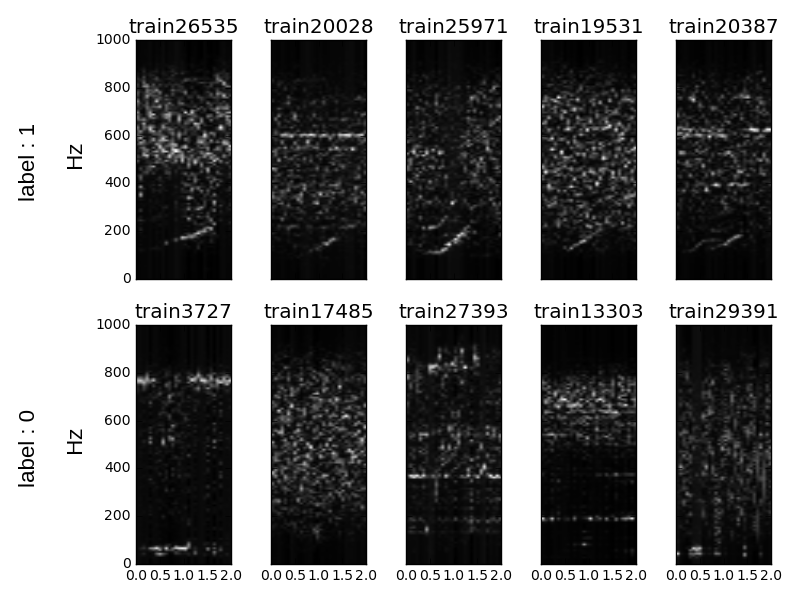
\includegraphics[width= \textwidth]{./images/2_samples_unprocessed}
\caption{ Samples after mean subtraction and division by standard deviation for right whale up-call (label 1) and no-right-whale up-call (label 0).  \label{img:samples_unprocessed}}
\end{figure} 

However, after applying this proccessing, images are not clear enough and energy where up-calls are contained is very low. In order to make them more visible, images in figure \ref{img:samples} are first processed applying log10 and then normalized subtracting mean and dividing by standard deviation.

\begin{figure}[htpb!]
\centering
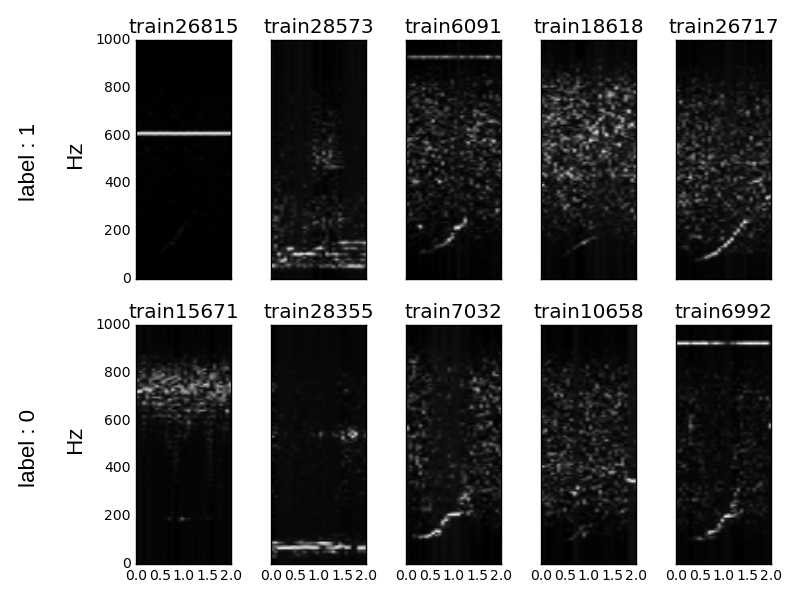
\includegraphics[width= \textwidth]{./images/2_samples_processed}
\caption{Processed samples after mean subtraction and normalization for right whale up-call (label 1) and no-right-whale up-call (label 0).  \label{img:samples_processed}}
\end{figure} 

As it was commented previously, recordings have a duration of 1.8 seconds and a sampling rate of 2000Hz. The raw spectrogram of the recordings result in images of 129x23 pixels. Two problems arise from this: the excess of redundant information in frequencies not important for the detection of the up-call and the limitation in terms of the image of being processed by the network.

In order to solve the first problem, the frequency range will be limited 0-250 Hz, what will result in images of size 33x23 px. Still, this is not good for a ConvNet with lots of convolutions and pooling. It is necessary to resize the image and a good number is multiple of 2. Hence, I will choose images to be 32x32 px and will obtain additional pixels using interpolation. %decir qué tipo de interpolación

\begin{figure}[htpb!]
\centering
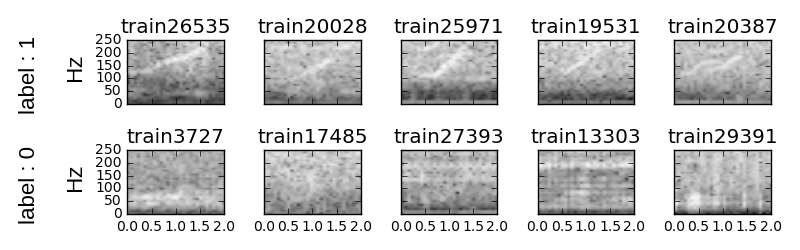
\includegraphics[width= \textwidth]{./images/2_samples_cropped}
\caption{Samples reduced to 32x32 pixels after log10 and mean subtraction and normalization for right whale up-call (label 1) and no-right-whale up-call (label 0).  \label{img:samples_processed}}
\end{figure} 


\subsubsection{Implementation}\label{implementation}
\begin{comment}
In this section, the process for which metrics, algorithms, and
techniques that you implemented for the given data will need to be
clearly documented. It should be abundantly clear how the implementation
was carried out, and discussion should be made regarding any
complications that occurred during this process. Questions to ask
yourself when writing this section: - \emph{Is it made clear how the
algorithms and techniques were implemented with the given datasets or
input data?} - \emph{Were there any complications with the original
metrics or techniques that required changing prior to acquiring a
solution?} - \emph{Was there any part of the coding process (e.g.,
writing complicated functions) that should be documented?}

            depth_1 = 6
            depth_2 = 6
            depth_3 = 16
            depth_4 = 16
            depth_5 = 120

            patch_size_1 = 5
            patch_size_2 = 2
            patch_size_3 = 6
            patch_size_4 = 2
            patch_size_5 = 6
\end{comment}
The model implemented is LeNet-5 (see figure \ref{img:lenet5}). The only difference in the F6 layer, which has been removed. This layer is used for the detection of ASCII characters in 7x12 bitmaps, but this network does not intend to do so, it just needs to detect right-whale up-call or not.

The structure of the network is as follows (F= Filter, S= Stride, D= Depth):
\begin{itemize}
	\item INPUT layer: 32x32 px image in grayscale represented with 8-bit number(0-255 levels).
	\item C1 - CONV layer: F = 5x5, S = 1, D = 6
	\item S2 - POOL layer: F = 2x2, S = 2, D = 6
	\item C3 - CONV layer: F = 5x5, S = 1, D = 16
	\item S4 - POOL layer: F = 2x2, S = 2, D = 16
	\item C5 - CONV layer: F = 5x5, S = 1, D = 120
	\item F5 - FC layer: neurons= 120 x 2, one per label(considering label 0 and label 1)
\end{itemize}

The training is performed using mini-batch gradient descent, which is a version of the true gradient descent, used when data amount is quite high. It iterates over batches in order to approach the minimum of the cost function step by step (epochs).

Regularization is a common way to prevent over-fitting and L2 regularization is the most used method. It penalized the square magnitude of all parameters, adding the term $\frac{1}{2}\lambda \omega ^2$ to the prediction, for $\lambda$ the regularization strength \cite{cs231convnets}. In this work L2 regularization will be used to control the over-fitting.

%L2-regularization 
\subsubsection{Select batch-size}
In order to select the proper batch size simulations have been performed for different learning rates.

\subsubsection{Select learning rate}
For a fixed batch size, the cost has been calculated for different learning rates.

\subsubsection{Select regularization}
For fixed batch size and learning rate , the cost has been calculated for different learning rates.

\subsubsection{Dropout and Batch normalization}


 
\pagebreak


\bibliography{../../../../../media/mabelvj/Darsena/DropboxUbuntu/Dropbox/PhD/library}

\end{document}
